\documentclass[11pt]{article}

\usepackage[landscape,margin=1.5cm]{geometry}
\usepackage{amsmath,amssymb}
\usepackage{array,tabularx}
\usepackage{pgfplots}
\usepackage{tikz}
\pgfplotsset{compat=1.18}

\renewcommand{\arraystretch}{1.6}
\setlength{\tabcolsep}{8pt}

\begin{document}

\begin{center}
\Large \textbf{Catálogo de Principales Distribuciones de Probabilidad}
\end{center}

%%%%%%%%%%%%%%%%%%%%%%%%%%%%%%%%%%%%%%%%%%%%%%%%%%
\section*{Distribuciones Discretas}

\small

\begin{tabularx}{\linewidth}{|
m{2.8cm}|
X|
m{1.8cm}|
m{2cm}|
m{2.3cm}|
m{4.2cm}|}
\hline
\textbf{Distribución} & \textbf{Función de densidad} & \textbf{Esperanza} & \textbf{Varianza} & \textbf{FGM} & \textbf{Gráfica} \\
\hline

Bernoulli &
$p^x(1-p)^{1-x}$ &
$p$ &
$p(1-p)$ &
$1-p+pe^t$
&
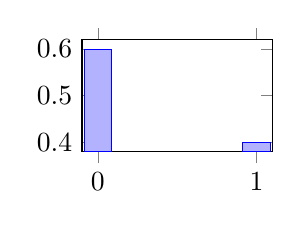
\begin{tikzpicture}
\begin{axis}[width=4cm,height=3cm,ybar,
symbolic x coords={0,1},xtick=data]
\addplot coordinates {(0,0.6)(1,0.4)};
\end{axis}
\end{tikzpicture}
\\
\hline

Binomial &
$\binom{n}{x}p^x(1-p)^{n-x}$ &
$np$ &
$np(1-p)$ &
$(1-p+pe^t)^n$
&
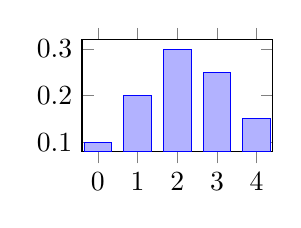
\begin{tikzpicture}
\begin{axis}[width=4cm,height=3cm,ybar,
symbolic x coords={0,1,2,3,4},xtick=data]
\addplot coordinates {(0,0.1)(1,0.2)(2,0.3)(3,0.25)(4,0.15)};
\end{axis}
\end{tikzpicture}
\\
\hline

Poisson &
$\frac{e^{-\lambda}\lambda^x}{x!}$ &
$\lambda$ &
$\lambda$ &
$e^{\lambda(e^t-1)}$
&
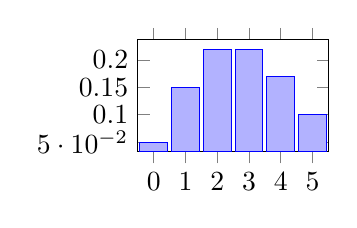
\begin{tikzpicture}
\begin{axis}[width=4cm,height=3cm,ybar,
symbolic x coords={0,1,2,3,4,5},xtick=data]
\addplot coordinates {(0,0.05)(1,0.15)(2,0.22)(3,0.22)(4,0.17)(5,0.10)};
\end{axis}
\end{tikzpicture}
\\
\hline

Geométrica &
$(1-p)^{x-1}p$ &
$\frac{1}{p}$ &
$\frac{1-p}{p^2}$ &
$\frac{pe^t}{1-(1-p)e^t}$
&
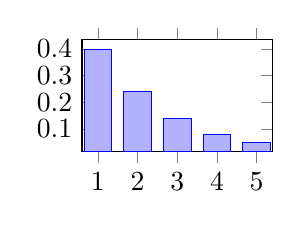
\begin{tikzpicture}
\begin{axis}[width=4cm,height=3cm,ybar,
symbolic x coords={1,2,3,4,5},xtick=data]
\addplot coordinates {(1,0.4)(2,0.24)(3,0.14)(4,0.08)(5,0.05)};
\end{axis}
\end{tikzpicture}
\\
\hline

Hipergeométrica &
$\frac{\binom{K}{x}\binom{N-K}{n-x}}{\binom{N}{n}}$ &
$n\frac{K}{N}$ &
$n\frac{K}{N}\frac{N-K}{N}\frac{N-n}{N-1}$ &
No simple
&
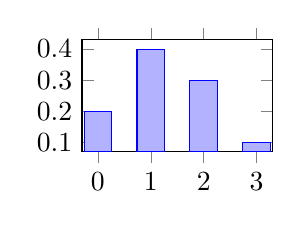
\begin{tikzpicture}
\begin{axis}[width=4cm,height=3cm,ybar,
symbolic x coords={0,1,2,3},xtick=data]
\addplot coordinates {(0,0.2)(1,0.4)(2,0.3)(3,0.1)};
\end{axis}
\end{tikzpicture}
\\
\hline

Binomial Negativa &
$\binom{x+r-1}{r-1}p^r(1-p)^{x}$ &
$\frac{r(1-p)}{p}$ &
$\frac{r(1-p)}{p^2}$ &
$\left(\frac{p}{1-(1-p)e^t}\right)^r$
&
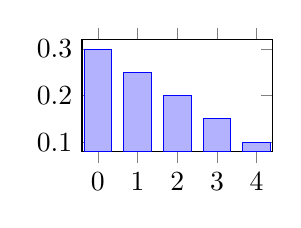
\begin{tikzpicture}
\begin{axis}[width=4cm,height=3cm,ybar,
symbolic x coords={0,1,2,3,4},xtick=data]
\addplot coordinates {(0,0.3)(1,0.25)(2,0.2)(3,0.15)(4,0.1)};
\end{axis}
\end{tikzpicture}
\\
\hline

\end{tabularx}

\newpage

%%%%%%%%%%%%%%%%%%%%%%%%%%%%%%%%%%%%%%%%%%%%%%%%%%
\section*{Distribuciones Continuas}

\small

\begin{tabularx}{\linewidth}{|
m{2.8cm}|
X|
m{1.8cm}|
m{2cm}|
m{2.3cm}|
m{4.2cm}|}
\hline
\textbf{Distribución} & \textbf{Funcion de densidad} & \textbf{Esperanza} & \textbf{Varianza} & \textbf{FGM} & \textbf{Gráfica} \\
\hline

Uniforme &
$\frac{1}{b-a}$ &
$\frac{a+b}{2}$ &
$\frac{(b-a)^2}{12}$ &
$\frac{e^{tb}-e^{ta}}{t(b-a)}$
&
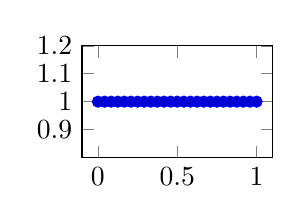
\begin{tikzpicture}
\begin{axis}[width=4cm,height=3cm,domain=0:1]
\addplot {1};
\end{axis}
\end{tikzpicture}
\\
\hline

Exponencial &
$\lambda e^{-\lambda x}$ &
$\frac{1}{\lambda}$ &
$\frac{1}{\lambda^2}$ &
$\frac{\lambda}{\lambda-t}$
&
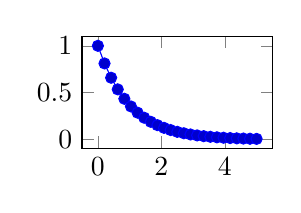
\begin{tikzpicture}
\begin{axis}[width=4cm,height=3cm,domain=0:5]
\addplot {exp(-x)};
\end{axis}
\end{tikzpicture}
\\
\hline

Normal &
$\frac{1}{\sigma\sqrt{2\pi}}e^{-\frac{(x-\mu)^2}{2\sigma^2}}$ &
$\mu$ &
$\sigma^2$ &
$e^{\mu t+\frac{\sigma^2t^2}{2}}$
&
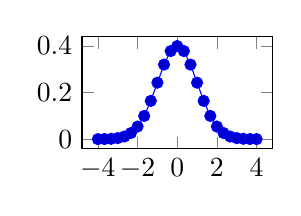
\begin{tikzpicture}
\begin{axis}[width=4cm,height=3cm,domain=-4:4]
\addplot {1/sqrt(2*pi)*exp(-x^2/2)};
\end{axis}
\end{tikzpicture}
\\
\hline

Chi-cuadrada &
$\frac{1}{2^{k/2}\Gamma(k/2)}x^{k/2-1}e^{-x/2}$ &
$k$ &
$2k$ &
$(1-2t)^{-k/2}$
&
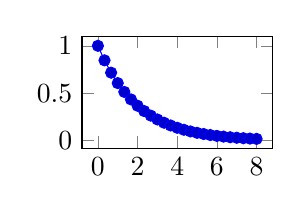
\begin{tikzpicture}
\begin{axis}[width=4cm,height=3cm,domain=0:8]
\addplot {x^(2/2-1)*exp(-x/2)};
\end{axis}
\end{tikzpicture}
\\
\hline

t Student &
$(1+x^2/\nu)^{-(\nu+1)/2}$ &
$0$ &
$\frac{\nu}{\nu-2}$ &
No existe
&
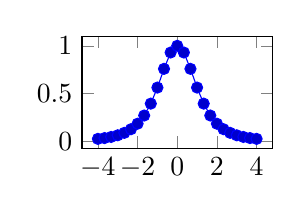
\begin{tikzpicture}
\begin{axis}[width=4cm,height=3cm,domain=-4:4]
\addplot {1/(1+x^2/3)^2};
\end{axis}
\end{tikzpicture}
\\
\hline

Gamma &
$\frac{\lambda^\alpha}{\Gamma(\alpha)}x^{\alpha-1}e^{-\lambda x}$ &
$\frac{\alpha}{\lambda}$ &
$\frac{\alpha}{\lambda^2}$ &
$(1-\frac{t}{\lambda})^{-\alpha}$
&
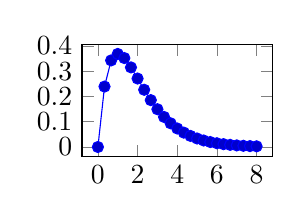
\begin{tikzpicture}
\begin{axis}[width=4cm,height=3cm,domain=0:8]
\addplot {x^(2-1)*exp(-x)};
\end{axis}
\end{tikzpicture}
\\
\hline

Beta &
$\frac{\Gamma(\alpha+\beta)}{\Gamma(\alpha)\Gamma(\beta)}x^{\alpha-1}(1-x)^{\beta-1}$ &
$\frac{\alpha}{\alpha+\beta}$ &
$\frac{\alpha\beta}{(\alpha+\beta)^2(\alpha+\beta+1)}$ &
No simple
&
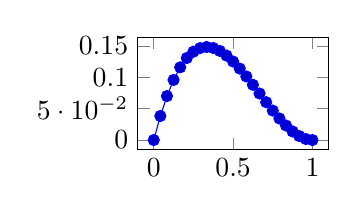
\begin{tikzpicture}
\begin{axis}[width=4cm,height=3cm,domain=0:1]
\addplot {x^(2-1)*(1-x)^(3-1)};
\end{axis}
\end{tikzpicture}
\\
\hline



\end{tabularx}

\end{document}